\chapter{Introduction}
Flow and transport processes between turbulent free-flows and porous-media 
flows 
are common in a wide range of environmental, industrial and medical 
applications. For example a turbulent air flow has a crucial effect on the 
drying rate of a wet porous-medium like a soil (see \cite{paper:fetzer}), or 
%Moreover when soils contain water with dissolved salts the evaporation can 
%induce the salt precipitation, which is problematic for the soil productivity, 
%and this is happening today in many areas of the world.
%inserire citazioe in riferimento alla salt precipitation.
in PEM (Proton Exchange Membrane) fuel cells transport phenomena through gas 
channels play an important 
role in the electrochemical reactions that determine the cell performances and 
efficiency (see \cite{wu:fuelcell}).

In order to study these processes we focus on the case of the evaporation from 
a soil surface and we consider a system that involves two subdomains: the upper 
one with a free-flow and the lower one occupied by a porous-medium. At the 
interface between the two subdomains there is exchange of mass, momentum and 
energy, but in the surrounding environment there is a great variety of 
phenomena that have an influence on these exchanges, as we can see for example 
in Figure~\ref{fig:intro}.
\begin{figure}[ht]
	\centering
	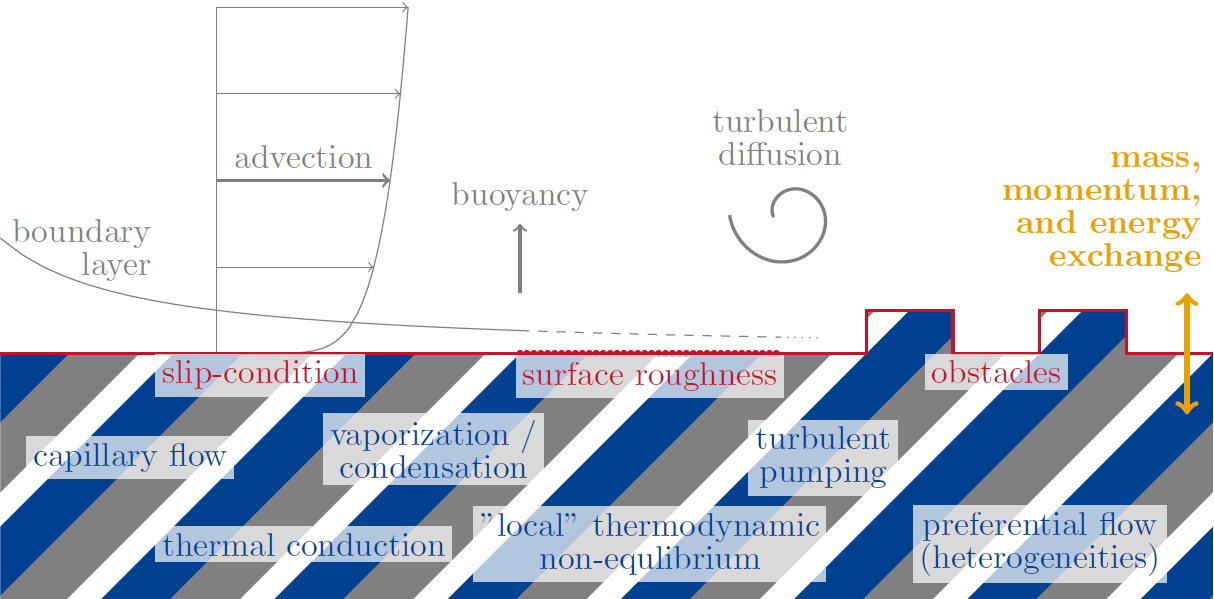
\includegraphics[width=\textwidth]{intropicture.png}
	\caption[Exchange processes between free and porous-medium 
	flows]{Example of physical phenomena affecting the exchange processes 
	between the free-flow and the porous-medium flow. Figure source: 
	\cite{tesi:fetzer}.}
	\label{fig:intro}
\end{figure}
Consequently a numerical study of this system generally involves a coupled 
model where the free-flow is described by the RANS equations and the 
porous-medium flow is described with a REV-scale approach, such as the Darcy's 
law. 
Simple models for single-phase systems can be generalized to take 
into account multicomponent non-isothermal flows, with one phase in the 
free-flow region and two phases in the porous-medium. Finally the problem 
has to be closed through suitable coupling conditions imposed at the 
interface; they are usually based on phenomenological arguments in order to 
keep the description simple and they should be as close as possible to the 
imposition of thermodynamic the equilibrium~\cite{paper:mosthaf}.

In this thesis the focus is on the improvement of the free-flow model. When the 
flow is in a turbulent regime, turbulent eddies develop near the interface and 
they cascade through consecutively smaller scales until the kinetic energy 
dissipates into internal thermal energy. Because of their location, they have 
a strong influence on the exchange processes between the two subdomains, so an 
accurate evaluation of their behaviour is of crucial importance. Improvements 
can be obtained of course with a refinement of the grid, but also employing 
high order methods; in 
particular, in the discretization of the Navier-Stokes equations using finite 
volumes, a key role is played by the approximation used for the non linear term 
$\nabla \cdot (\mathbf{v} \mathbf{v}^\mathrm{T})$. A common and easy 
choice is to employ a first order upwind approximation for the 
\emph{transported} velocity, but this option can produce solutions with a lot 
of numerical diffusion. Other possibilities are given by high order methods 
like the Linear Upwind Differencing (LUD) scheme, the Central Differencing (CD) 
scheme or the Quadratic Upstream Interpolation for Convective Kinetics (QUICK) 
scheme; sometimes they can produce 
accurate solution but they have also shown to be not stable in certain 
situations and to produce overshoots or undershoots that 
may lead to unphysical values of quantities that for example have to be 
positive (see \cite{main:vermal}). With this in mind our interest will in be in 
the Total Variation Diminishing (TVD) methods, a family of methods that has 
been derived with the purpose of providing a solution with a second order 
accuracy, but without any risk of numerical oscillations. They are called also 
high resolution methods.

In Chapter~\ref{chap:equations} the equations employed in the models will be 
presented, with particular attention to the free-flow equations. In 
Chapter~\ref{chap:discretization} the finite volume method will be described 
and in Subsection~\ref{subsec:tvd} the TVD methods will be introduced. At last, 
in Chapter~\ref{chap:results}, the numerical results will be shown; in 
particular we will see the application of the TVD methods to the Navier-Stokes 
equations in comparison to the first order upwind scheme, then two tests 
involving turbulent flows and finally a more complex scenario involving 
obstacles at the interface between a free-flow region and a porous-medium.

The high order methods mentioned above have been implemented in the framework 
of the open-source simulator \DUMUX: DUNE for multi-$\{$phase, component, 
scale, physics, \dots$\}$ flow in porous-media, see \cite{dumux:tutti} and 
\cite{dumux:flemisch}. \DUMUX is an 
additional module of DUNE (Distributed and Unified Numerics Environment, 
\cite{web:dune}) and, through the use of an object-oriented design in 
conjunction with template programming, it provides a C++ environment that 
allows 
an efficient implementation of numerical models related to porous-media flows.

All the source code used for the simulations performed can be 
found at \url{https://git.iws.uni-stuttgart.de/dumux-pub/vescovini2019a}, 
together with the instructions to install the required software.